\subsection{TAOCP 7.1.3 Exercise 198, UTF-8 encoding and program synthesis by sketching}

Found this exercise in TAOCP 7.1.3 (Bitwise Tricks and Techniques):

% TODO: border
\begin{figure}[H]
\centering
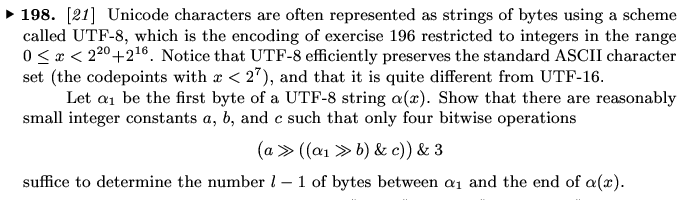
\includegraphics[scale=0.75]{pgm_synth/TAOCP_713_198/TAOCP_713_198.png}
\caption{Exercise from TAOCP book}
\end{figure}

This is like program synthesis by sketching: you give a sketch with several ``holes'' missing and ask some
automated software to fill the ``holes''.
In our case, $a$, $b$ and $c$ are ``holes''.

Let's find them using Z3:

\lstinputlisting[style=custompy]{pgm_synth/TAOCP_713_198/198.py}

I tried various bit widths for a, b and c and found that 22 bits are enough.
I've lots of results like:

\begin{lstlisting}
...

a,b,c = 0x250100 0x3 0x381416
a,b,c = 0x258100 0x3 0x381416
a,b,c = 0x258900 0x3 0x381416
a,b,c = 0x250900 0x3 0x381416
a,b,c = 0x251100 0x3 0x381416
a,b,c = 0x259100 0x3 0x381416
a,b,c = 0x259100 0x3 0x389416
a,b,c = 0x251100 0x3 0x389416
a,b,c = 0x251100 0x3 0x189416
a,b,c = 0x259100 0x3 0x189416
a,b,c = 0x259100 0x3 0x189016

...
\end{lstlisting}

It seems that several least significant bits of a and c are not used.
After little experimentation, I've come to this:

\begin{lstlisting}
...

# make a,c more aesthetically appealing:
s.add((a&0xffff)==0)
s.add((c&0xffff00)==0)

...
\end{lstlisting}

And the results:

\begin{lstlisting}
a,b,c = 0x250000 0x3 0x36
a,b,c = 0x250000 0x3 0x16
a,b,c = 0x250000 0x3 0x96
a,b,c = 0x250000 0x3 0xd6
a,b,c = 0x250000 0x3 0xf6
a,b,c = 0x250000 0x3 0x76
a,b,c = 0x250000 0x3 0xb6
a,b,c = 0x250000 0x3 0x56
results total= 8
\end{lstlisting}

Pick any.

But how it works?
Its operation is very similar to the bitwise trick related to leading/trailing zero bits counting based on De Bruijn sequences.
Read more about it:
\url{https://yurichev.com/blog/de_bruijn/},
\ref{DeBruijnZ3}.

